\chapter{The SMBO Paradigm}\label{ch:smbo}

To formalize the notion of blackbox optimization, consider an expensive blackbox function $f$. I will also refer to $f$ as the \emph{objective function}, a term from the optimization and statistics communities. Say that $f$ has been evaluated on the inputs, or \emph{sample points}, $x^1,\ x^2, ... ,\ x^n$. These evaluations produce the observed outputs $y^i=f(x^i)$. If $\X=\{x^1, ... ,\ x^n\}$ and $\Y=\{y^1, ...,\ y^n\}$, I'll refer to the pair $(\X,\Y)$ as the \emph{sample data}. Because we are concerned with global optimization---without loss of generality, say minimization\footnote{In the optimization community, it is common to speak only of minimization, and the two words are used somewhat interchangeably. For example, the most popular Python library for optimization, \texttt{scipy.optimize}\cite{scipy_optimize}, contains only minimization routines. Of course, the task of maximizing a function $f$ is the same as minimizing its negative $-f$. }---the goal is to find an $x$ such that $f(x)<f(x')$ for all $x' \ne x$, while evaluating $f$ as few times as possible. This chapter describes formally how the SMBO process addresses this challenge. I will define notation as it is introduced, though for reference I have included a reference table of variable names and definitions in Figure \ref{fig:notation} below.
% Where does this important aside go?: It should be clear that, unless you have evaluated the black box function $f$ at every possible $x$, it is impossible to say with absolute certainty whether a given point is the global minimum. Thus, the goal of a statistical global optimization routine is to produce a candidate optimum $x$, with some measure of confidence that $x$ is in fact the global optimum.

\begin{minipage}{\textwidth}
\begin{framed}
\begin{description}[leftmargin=!,labelwidth=\widthof{\bfseries thre}]
  \item[$f$]: the objective function
  \item[$k$]: the dimensionality of $f$'s domain
  \item[$x$]: a generic point in $f$'s domain
  \item[$x^i$]: the $i$th sample point(a $k$-vector)
  \item[$n$]: the number of sample points
  \item[$\X$]$=\{x^1,x^2,...,x^n\}$, the input vector
  \item[$y^i$]$= f(x^i)$; the known objective output at the $i$th sample point (a real number)
  \item[$\Y$]$=\{y^1,y^2,...,y^n\}$, the output vector
  \item[$\hat{f}(x)$]: the predictor function
  \item[$s^2(x)$]$=s(x)^2$, the estimated variance of the prediction $\hat{f}(x)$.  
  \item[$y(x)$]: a random variable with expected value $\hat{f}(x)$ and variance $s^2(x)$, representing the prediction at $x$.
\end{description}


\end{framed}
\captionof{figure}{Reference table for SMBO notation}
\label{fig:notation}
\end{minipage}

\section{The SMBO Loop}

`SMBO' describes an entire class of algorithms, rather than one in particular \footnote{\cite{hutter_sequential_2011, hamadi_autonomous_2012, jones_efficient_1998, rasmussen_gaussian_2006}}. %note: get more specific with those cites. should be a handful of specific papers presenting particular SMBO things
These algorithms differ along several dimensions: in their assumptions regarding determinism, the types of objective functions they can optimize, their modelling strategies, and the details of their interactive relationship to the objective functions being optimized, to name several. % clarification: such as some algorithms selecting one sample point, others more.
Across these differences, the defining feature of sequential model-based optimization can be described as a three-part loop, shown below. I'll call this three-part process the \emph{SMBO loop} or \emph{cycle}; it will be referenced throughout this thesis. 


\begin{minipage}{\textwidth}
\begin{framed}

\begin{enumerate} 
\item The objective function $f$ is evaluated at a set of input values $\X$, producing observed outputs $\Y$.
\item A prediction model of the objective function, the ``predictor function'' $\hat{f}$ is fit to the sample points $(\X,\Y)$, as well as a model of the expected variance of $\hat{f}$, $\err$.
\item From considering the prediction surface and its error, $(\hat{f},\err)$, $m$ new input points $x^{n+1},...,x^{n+m}$ are chosen to be evaluated by $f$. These points are chosen to most improve the ability of the model $(\hat{f},\err)$ to find the global optimum.\end{enumerate}
\end{framed}

\captionof{figure}{The three-stage SMBO loop}
\label{fig:smbo_loop}
\end{minipage}


Note that at every iteration of the SMBO loop, (presuming we are minimizing $f$) there is a current `incumbent minimum', the best sample point evaluated so far. I will denote this point $x_{min}$, and use $y_{min}$ to denote the current best output $f(x_{min})$.

The SMBO loop returns $(x_{min},y_{min})$ once $y_{min}$ represents a satisfactory optimization result. As will be described further in Section \ref{sec:max_imp}, we can construct from the prediction model $(\hat{f},\err)$ a rigorous metric called `expected improvement', which lends to several reasonable stopping criteria, such as, ``return $y_{min}$ when you are 95\% confident that it is indeed the global minimum,'' or ``return $y_{min}$ when you are 95\% confident that it is within $\alpha$ of the global minimum.''

\section{Visualizing the SMBO Loop}

The cyclical nature of sequential model-based optimization suggests a popular illustration of the method, which highlights how the three steps reinforce each other to generate successively more predictive models---see Figure \ref{fig:smbo_cycle}, below. It is somewhat notable that illustrations quite similar to Fig. \ref{fig:smbo_cycle} appear throughout the literature related to SMBO, such as \cite{hutter_sequential_2011} and \cite{protolife_pdt_2013}. This image is perhaps the most popular conceptualization of the SMBO method.

\begin{figure}[h]
	\centering
	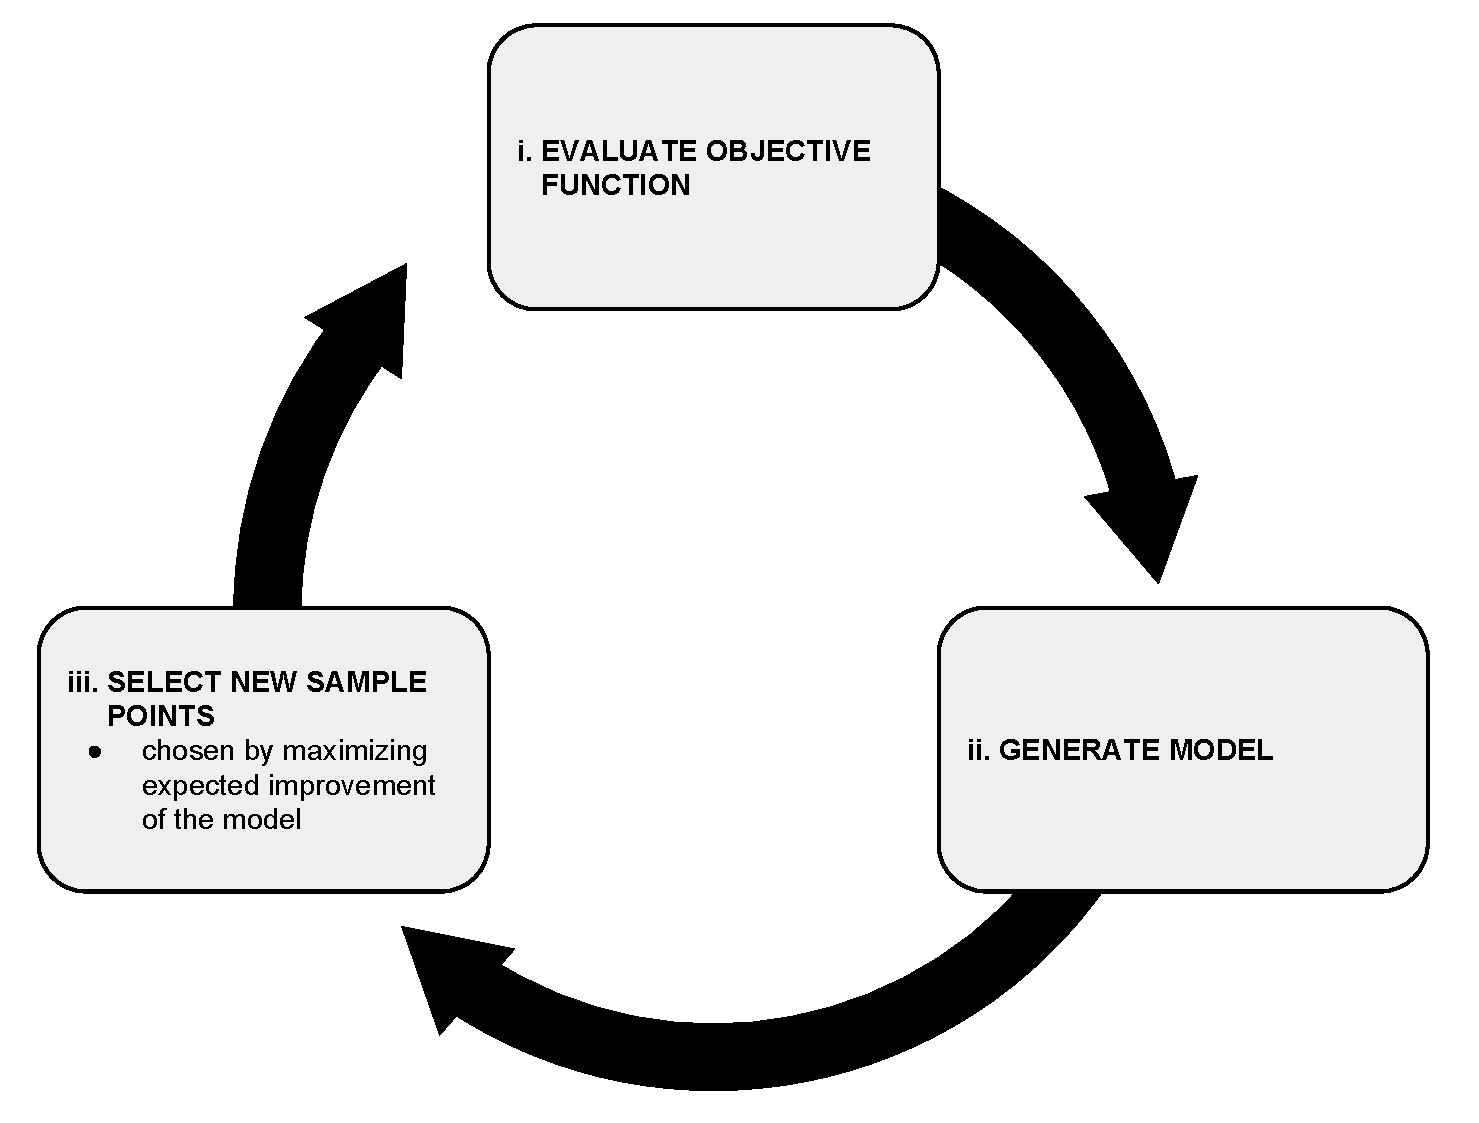
\includegraphics[width=0.75\textwidth]{images/smbo_loop}
	\caption{A popular visualization of SMBO as a three-part loop.}
	\label{fig:smbo_cycle}

\end{figure}


%In the vocabulary of above, each stage in the SMBO loop can be defined as a mathematical function:
%\begin{description}
%	\item[\textbf{I}]: The objective function maps $k$-vectors from input-space to outputs.
%	\item[\textbf{II}]: The model module maps the sample points to a model function.
%	\item[\textbf{III}]: The sampling strategy is a function that takes as input a model function, and outputs the next $k$-vector(s) which should be evaluated by the objective.
%\end{description}

%Seeing each component as simply a function mapping a certain kind of input to a certain kind of output, combined with the circular relationship illustrated in Fig \ref{fig:smbo_cycle}, is what motivates me to describe the SMBO process as bootstrapping. From the perspective of node \textbf{I} in the cycle, the output of the objective function determines the next input of the objective function, which determines the next input, and do on. From the perspective of node \textbf{II}, each model induces the model that follows it.

\section{SMBO Step III: Maximizing Improvement}\label{sec:max_imp}

The first step of the SMBO loop is defined by the optimization problem at hand. An interesting feature of SMBO is that a wide variety of modelling methods could be used in the second step of the loop; I will discuss the DACE method used by EGO in particular in the next chapter, and mention several others in Chapter \ref{ch:discussion}. There is a method used to perform third step, though, that is widespread enough, and interesting enough, to merit discussion here: choosing further sample points by maximizing a function of input space called \emph{expected improvement}. 

In global search problems such as optimization, it is commonly said that one needs to balance the competing search criteria of exploration and exploitation. Here, exploration refers to the impulse to investigate unknown regions of the objective function's domain, to learn more about its global behavior. Exploitation means the impulse to take advantage of what we already know, and sample where we currently predict that the global phenomenon's behavior is most desirable. At first, these seem like fairly opposite concepts, but expected improvement is one of those results from statistics that manages to quantify something you didn't think could be quantified. As we will see, choosing sample points to maximize the expected improvement of our model provides a very satisfying solution to the exploration/exploitation conundrum.

Remember that during the SMBO process (as in many other optimization strategies), there is at all times a current ``incumbent minimum,'' $(x_{min},y_{min})$, which is the most optimal sample point evaluated so far. Simply put, the expected improvement of $x$ measures the amount by which we predict that the objective value at $x$ would be more optimal than $y_{min}$. Consider the random variable $y(x)$, which has expected value $\hat{f}(x)$ and variance $s(x)$. Improvement $I$ is then defined as,

\begin{equation} \label{eq:improvement}
I(x) = max(y_{min}-y(x),0).
\end{equation}
$I$ is a random variable defined in terms of the random variable $y(x)$, so we can use standard statistical methods to derive its expected value $\mb{E}[I(x)]$ in terms of $\hat{f}(x)$ and $\err(x)$---this is how we define the expected improvement at $x$. Observe that finding the expected value of $I(x)$ encodes our prediction of how much our current optimum $y_{min}$ would improve if we were to sample $f$ at $x$.

From this definition of improvement, all that is left is to apply the basic statistical notion of the expected value of a random variable to Eq. \ref{eq:improvement} to find the expected improvement function $\mb{E}[I(x)]$. Doing this, along with what \cite{jones_efficient_1998} calls `some tedious integration by parts,' produces the formula,

\begin{equation} \label{eq:exp_improvement}
\mb{E}\left [I(x)\right ]=(y_{min}-\hat{f}(x))\cdot\Phi\left(\frac{y_{min}-\hat{f}(x)}{s(x)}\right) + s(x)\cdot\phi\left(\frac{y_{min}-\hat{f}(x)}{s(x)}\right),
\end{equation}
where $\phi$ and $\Phi$ denote the standard normal p.d.f. and c.d.f., respectively.

A significant feature of expected improvement is that it is monotonic in both $s$ and $\hat{f}$. Ignoring $\hat{f}(x)$, if the prediction at $x$ has a high variance, then the expected improvement at $x$ will be large---this incentivizes exploration, because prediction error is usually largest in regions farthest from existing sample points. On the other hand, if we ignore prediction error, it is obvious that the points in domain where $\hat{f}(x)$ is lower will have a higher expected improvement (assuming the goal is minimization). This encodes the drive for exploitation. Thus, by choosing sample points to maximize the expected improve function, exploration and exploitation go hand in hand, and we quantify an intuitive measure of how much our optimization project might benefit from sampling at $x$. This feature of SMBO is especially visible in the example I will present in Section \ref{sec:smbo_ex}.

\section{The Loop's $0^{th}$ Step: The Initial Sample}\label{sec:lh}

Obviously, it is impossible to construct a model of a blackbox function's response surface if you have not ever queried the function at all, so the SMBO loop cannot start itself without a strategy for picking an initial set of sample points. This is a brief and technical detail, not of particular theoretical interest to this thesis; the more theoretically-inclined reader might choose to skip over this section to the example presented in Section \ref{sec:smbo_ex}.

A popular strategy for selecting these points, and the only strategy I will consider in this thesis, is called a latin hypercube sample. To construct an $n$-point latin hypercube in $k$ dimensions, first divide each dimension's domain into $n$ rows, creating an $n^k$-cell grid of rectangular subdomains of $f$. The idea in latin hypercube sampling is that along any one dimension, there is exactly one sample in each row. Other than that, samples are chosen randomly. Sampling is then a two-step process: first, you randomly choose which $n$ of the $n^k$ cells will be occupied by samples under the latin hypercube constraint, and then locate each sample randomly from its assigned cell.


Ignoring the position of samples within their cells, but considering only the distribution of which $n$ cells in the $n\times n \times...\times n$-cell grid are occupied, we find some interesting combinatorial properties, and analogies to two popular games. If you are a fan of sudoku, you have spent a lot of time thinking about this distribution: the arrangement  of any one numeral across the game board matches a nine-sample latin hypercube in two dimensions\footnote{Though not all $(9,2)$ latin hypercubes represent a legal distribution of one numeral on a sudoku board; the explanation of this is left as an exercise to the reader.}, as shown in Figure \ref{fig:sudoku}. In a similar vein, imagine a chess board with only eight rooks on it, each rook hostile towards all the others, arranged such that no two rooks are threatening each other. The set of $n$-point latin hypercubes in $k$-dimensions is basically identical to the set of non-threatening arrangements of $n$ mutually-hostile hyperrooks on the $n\times n \times...\times n$ ($k$ dimensional) chess board.

\begin{figure}[h]
\centering
\includegraphics[width=\textwidth]{images/sudoku2}
\caption{The positions of one numeral on a complete sudoku board form a $9$-point latin square; e.g. the 3s above show a possible initial sampling of a 2D optimization domain. }
\label{fig:sudoku}
\end{figure}


\section{A First Example}\label{sec:smbo_ex}

To build the reader's intuition about the process of sequential model-based optimization, I will here present plots illustrating the minimization of a simple 1D toy problem using SMBO. These plots will show the EGO algorithm in particular, which I will present in detail in Chapter \ref{ch:ego}, but the features of interest are common to all SMBO processes. The plots were generated by my SMBO Python package, \texttt{smbo}, which is presented in Chapter \ref{ch:code}.

For our toy problem, consider a 1D blackbox function $f$ over the domain $[0,10]$. In order to begin the SMBO process of optimizing this function, we must choose an initial set of sample points $\X$ at which to query $f$, to form the starting data set $(\X,\Y)$. The details of this selection are not of particular conceptual significance, and are discussed in Section \ref{sec:lh}. For now, assume we have selected 8 points roughly at random from throughout $f$'s domain, and evaluated $f$ at each one, thus gathering the initial data set $(\X,\Y)$ plotted below in Figure \ref{fig:first_step}(a).



\begin{figure}[width=\textwidth]
\centering
\begin{tabular}{lr}

\subcaptionbox{The initial sample $(\X,\Y)$ of our toy blackbox function}
{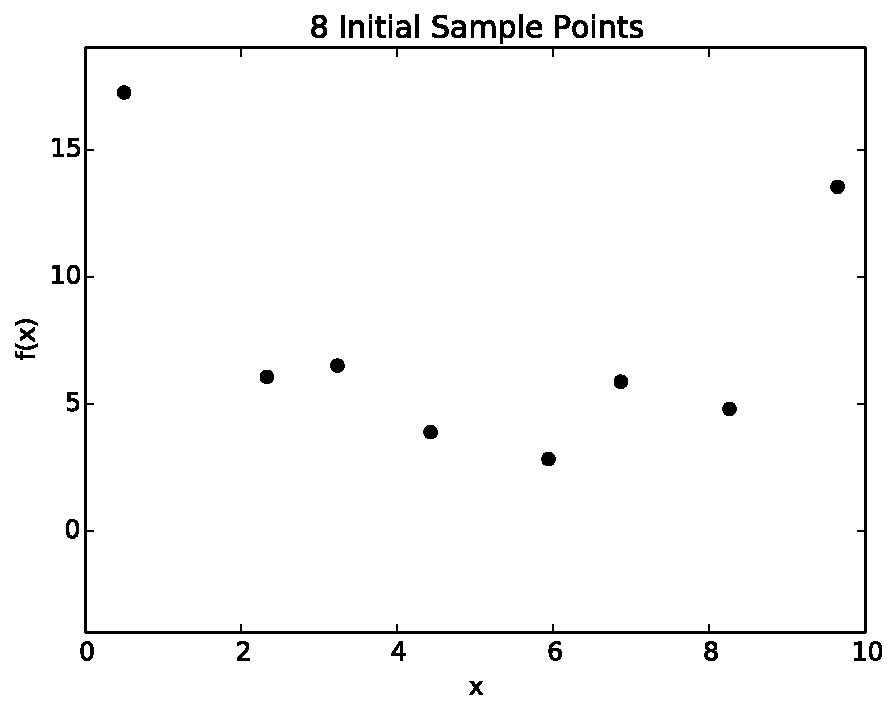
\includegraphics[width=0.45\textwidth]{images/ego_ex/just_points}}\label{fig:samp_data}
 &

\subcaptionbox{The EGO algorithm's predictive model $\hat{f}\pm \mb{s}(x)$ fit to our initial sample}
{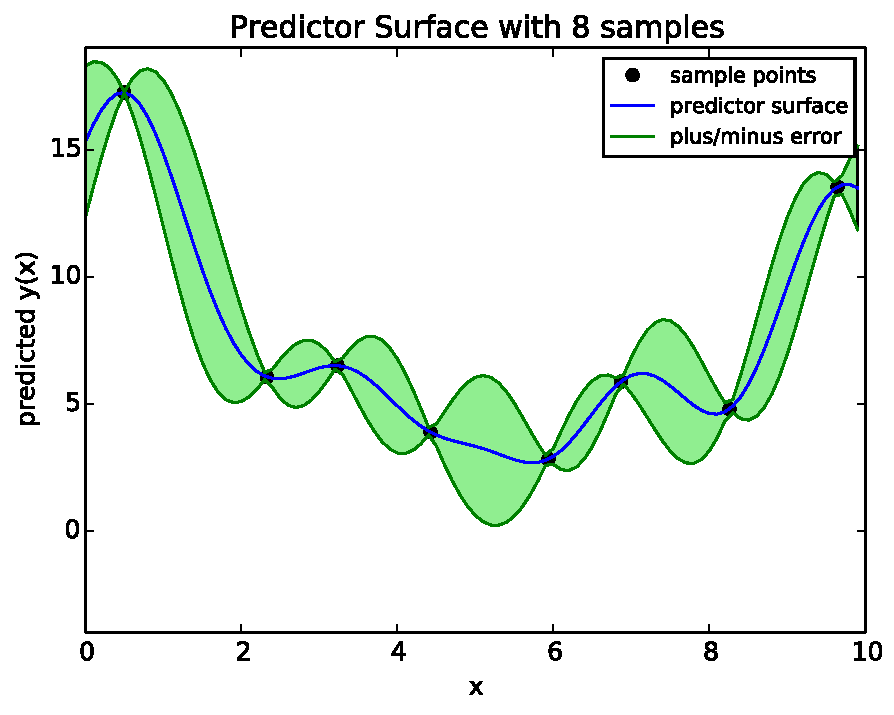
\includegraphics[width=0.45\textwidth]{images/ego_ex/just_pred}} \\
\end{tabular}
\caption{The first step of our sequential model-based optimizer\\}

\label{fig:first_step}
\end{figure}

These data constitute the first step of the first round of SMBO---the objective function has been evaluated at the initial sample points. From looking at this first data set, we notice that generally, the inputs closer to the middle of the domain $[0,10]$ have lower function values. Recalling our assumption (consistent throughout this thesis) that the blackbox function $f$ is both deterministic, another striking feature we learn from the data is that there are at least three local minima: counting from the left (and starting at one), sample points 2, 5, and 7 all have lower $f$ values than their neighbors.



Now, it is time for the second step of the loop, to fit a predictive model to the data. Regardless of the particular SMBO process being used, step two of the loop produces a predictor function and a measure of its expected error. Plotted in Figure \ref{fig:first_step}(b) are these two functions as they are set in the EGO algorithm, whose specifics I will describe in-depth in the next chapter. Illustrating both the prediction surface and its standard error, the figure highlights the probabilistic nature of the prediction models used in the second step of the SMBO loop.

Figure \ref{fig:first_impv} summarizes the first two steps of the SMBO loop: the gathering of objective data, and the fitting of a model function to that data. Note that the predictor error is zero at each sample point, because we know that $f$ is deterministic, and so we can predict $f(x^i)$ for each sample point $x^i$ with total certainty. Under the EGO model shown here, predicted error $\err(x)$ increases as a function of $x$'s distance from nearby sample points. This is visible as a sort of `error ballooning' of the prediction between the samples. Clearly, the prediction is most uncertain in those places in the domain $[0,10]$ that are farthest from the already-sample points.


Using the model produced in step two, we now choose the next sample point to evaluated by the blackbox function $f$, by maximizing the expected improvement function \footnote{Eq. \ref{eq:exp_improvement}} over the domain \footnote{as described in Section \ref{sec:max_imp}}. Building on the previous figures, the expected improvement function is overlaid in red in Figure \ref{fig:first_imp}. The vertical dashed line highlights the global maximum of this expected improvement function, which is chosen as the next sample point.

\begin{figure}[h!]
\centering
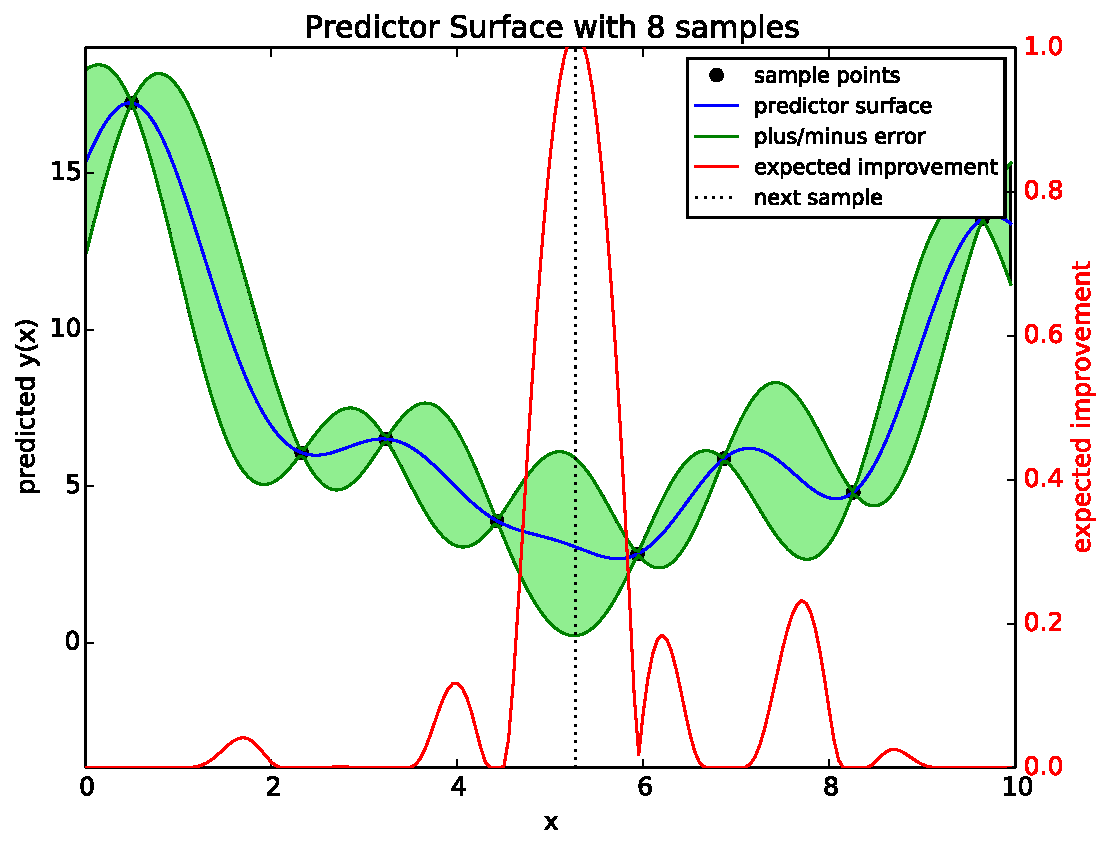
\includegraphics[width=0.6\textwidth]{images/ego_ex/0}
\caption{A plot of the entire initial SMBO loop of our toy problem\\}
\label{fig:first_imp}
\begin{minipage}{\textwidth}

\ \\ Figure \ref{fig:first_imp} plots an entire SMBO loop. Note that the next sample, marked with the vertical dotted line, intuitively serves both goals of exploration and exploitation---it lies in a region where both the predictor function $\hat{f}(x)$ is low, and the error of that prediction $\err(x)$ is high (visualized by the height of the green error envelope). This $x$ is not only a decent guess of where a global minimum might lie, it also lies approximately in the middle of a relatively large unexplored region of the domain. Sampling at $x$ is a smart decision such that the next model we will make, with $(x,f(x))$ added to $(\X,\Y)$, will tell us more about where the location of the global minimum.\\

Having now built up an all-in-one SMBO loop plot piece by piece, I will show similar plots for the rest of the SMBO loops in this optimization, so we can see how the process evolves and accomplishes its task. Formatting will be slightly abnormal the sake of keeping discussion on the same page as the relevant figures.


\end{minipage}

\end{figure}




\begin{figure}
\centering
\begin{tabular}{lr}

\subcaptionbox{}
{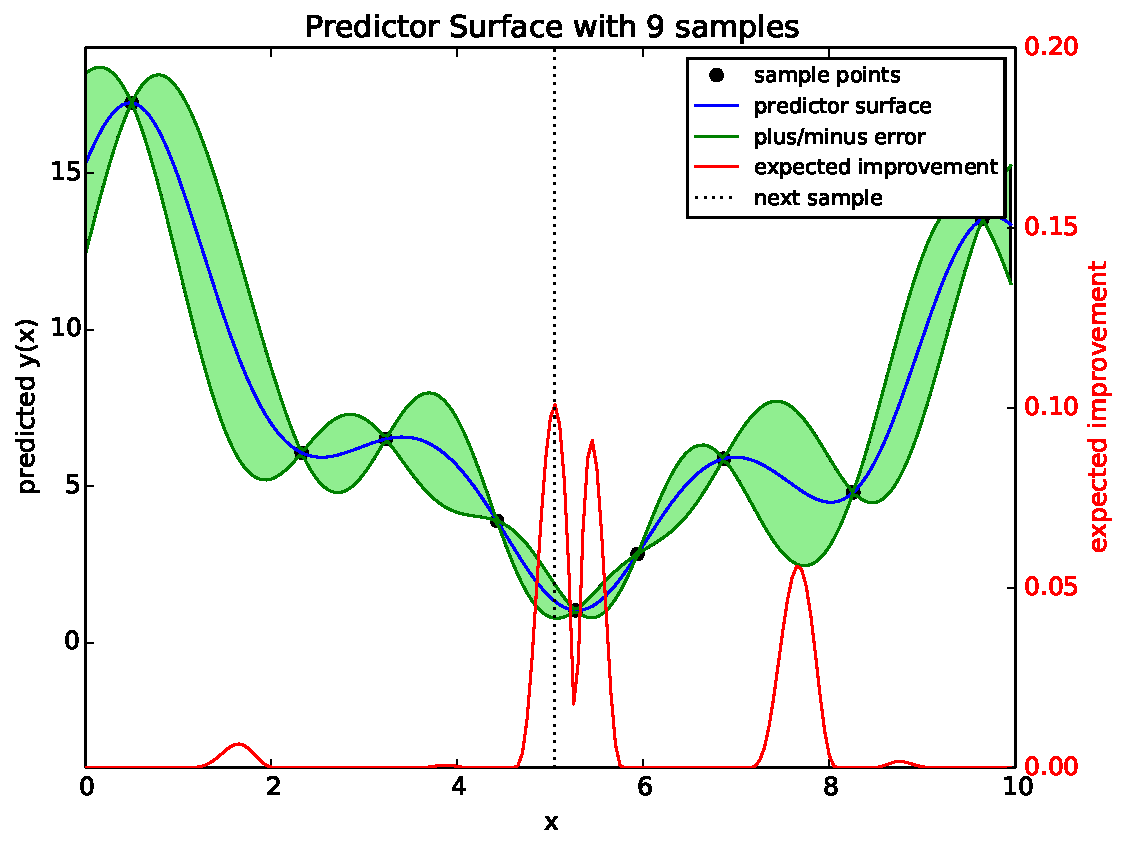
\includegraphics[width=0.45\textwidth]{images/ego_ex/1}} &

\subcaptionbox{}
{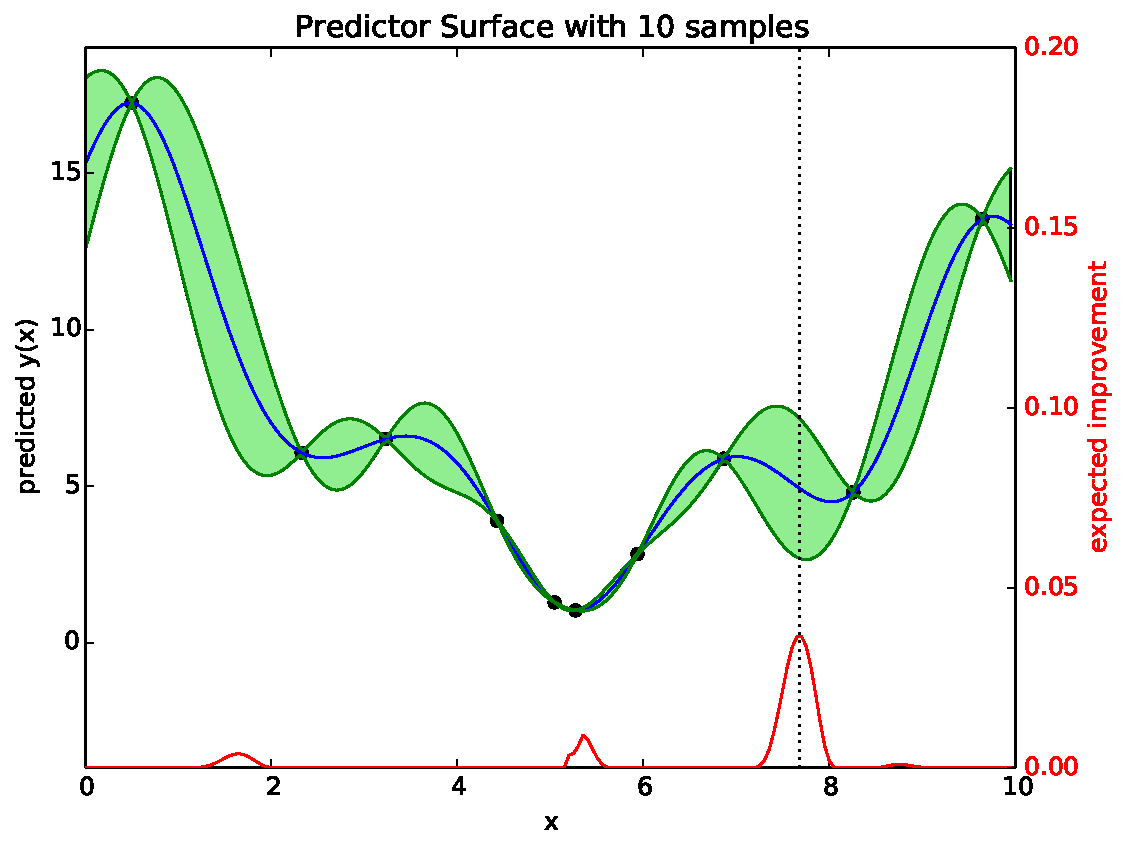
\includegraphics[width=0.45\textwidth]{images/ego_ex/2}} \\
\end{tabular}
\caption{The first and second SMBO loops of our toy problem. The first sample appears to be chosen to exploit; the second, to explore.\\}


\begin{minipage}{\textwidth}

The new sample chosen by the initial SMBO loop, around $x=5$ in (a), has shown to be a very good choice indeed, and is now the new \emph{incumbent minimum}, the best sample seen so far. After the first loop (imagining that the initializing loop in Fig. \ref{fig:first_imp} was the zeroth), we see that the maximum expected improvement criterion selects another point near this incumbent to investigate, looking near the current optimum to see if it can find an even better solution. \\

After sampling at this new point, (b) shows that the objective function value there was in fact less optimal than the incumbent. With relatively many samples in a small region of the domain, the error of the prediction is now very low in the area around the incumbent solution, from about $x=4$ to $x=6$. At this point, the next sample chosen by maximum expected improvement is fairly distant, lying near the middle of a large unsampled area.\\

Note that we have zoomed in on the vertical axis of the expected improvement plot has zoomed in since Figure \ref{fig:first_imp}.

\end{minipage}


\label{fig:explore_exploit}
\end{figure}


\begin{figure}[h]
\centering
\begin{tabular}{lr}
\subcaptionbox{}
{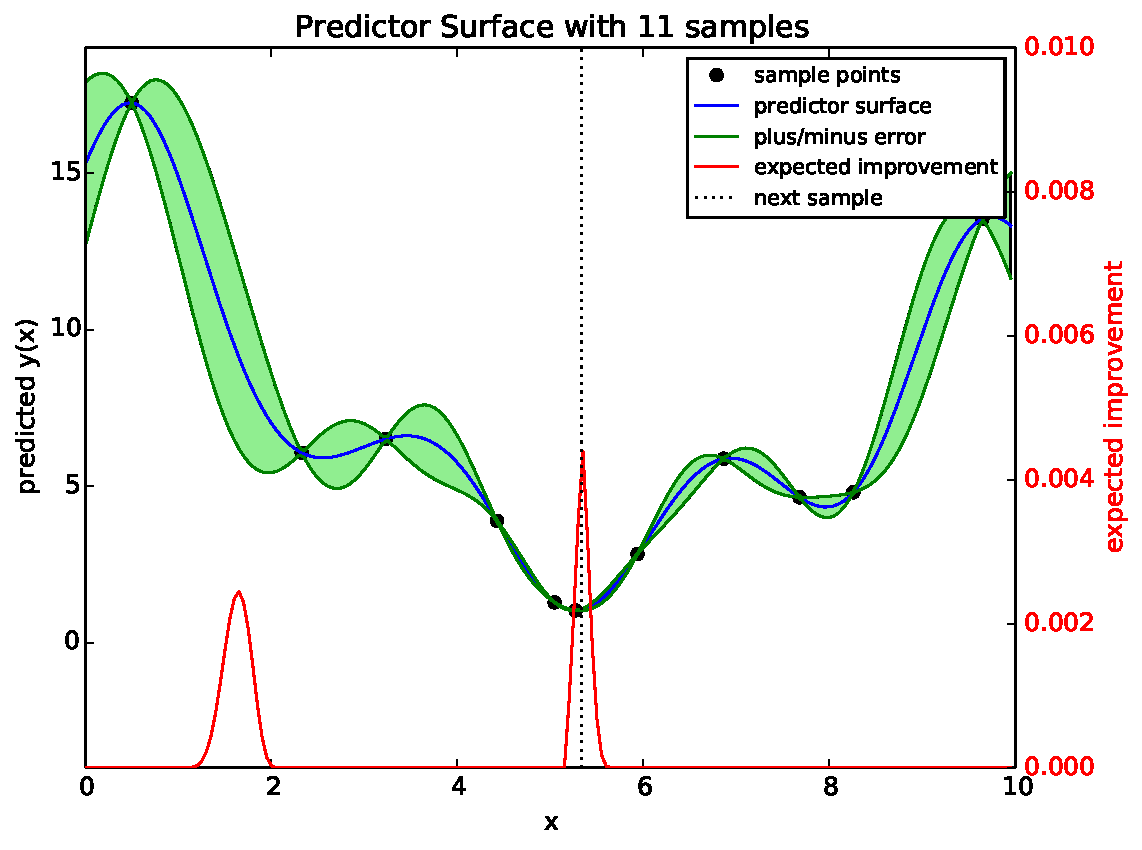
\includegraphics[width=0.45\textwidth]{images/ego_ex/3}} &

\subcaptionbox{}
{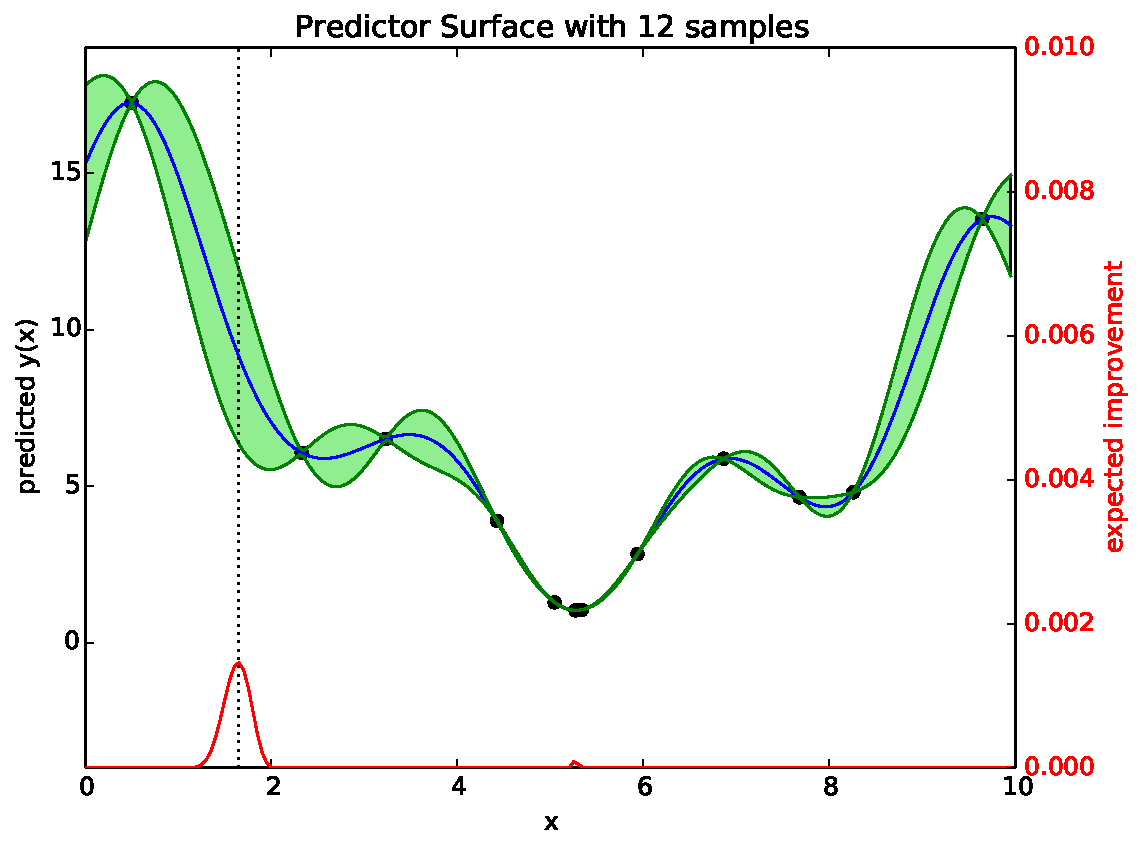
\includegraphics[width=0.45\textwidth]{images/ego_ex/4}} \\
\end{tabular}
\caption{The third and fourth iteration of the SMBO loop on the toy problem\\}
\label{fig:explore_exploit}

\begin{minipage}{\textwidth}

\ \\Again, zooming in on the vertical axis of the expected improvement plot, our $x_{new}$ criterion returns the search to the area around the incumbent. Adding this sample point, we find that maximum expected improvement sends us right back into the hinterlands of $f$'s domain, to explore the largest remaining unsampled region.\\

In (b) above, the expected improvement has already become quite small across the domain, after only 4 rounds of model-fitting. The optimization process is nearly complete.

\end{minipage}

\end{figure}




\begin{figure}[h]
\centering
\begin{tabular}{lr}
\subcaptionbox{}
{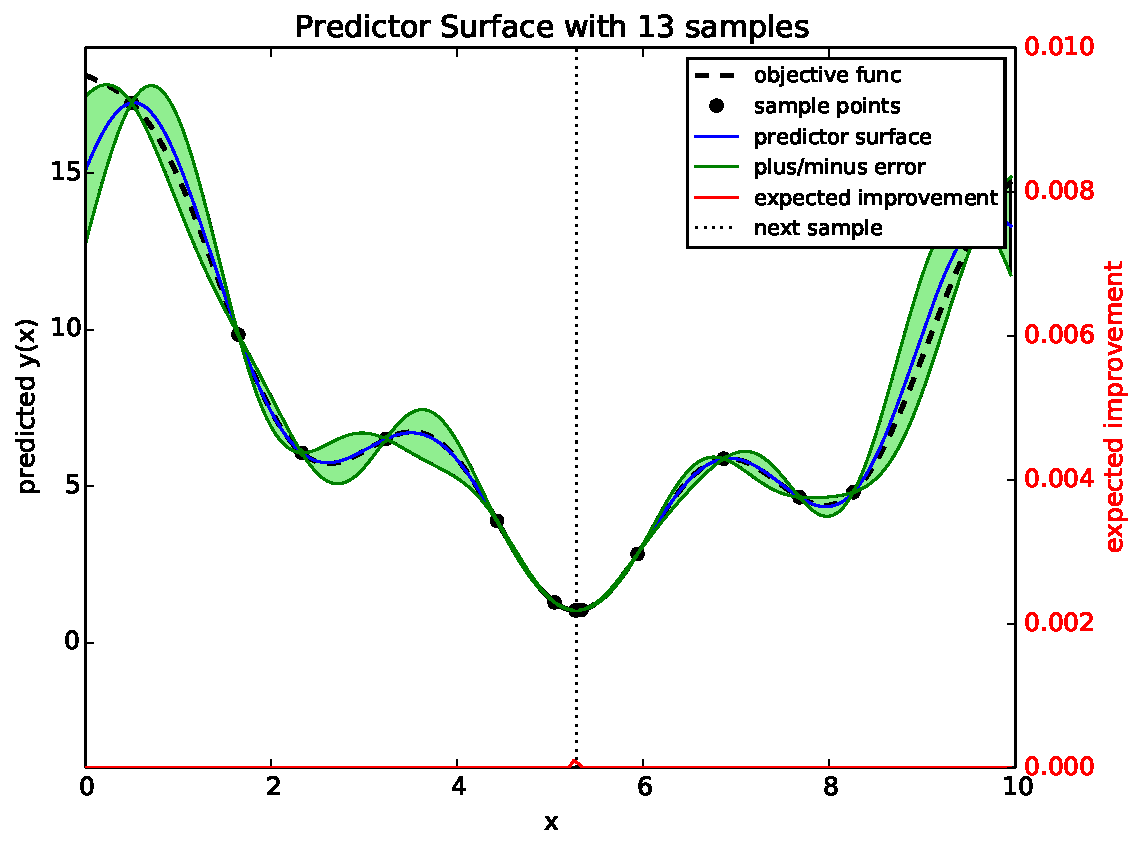
\includegraphics[width=0.5\textwidth]{images/ego_ex/5}} &

\subcaptionbox{}
{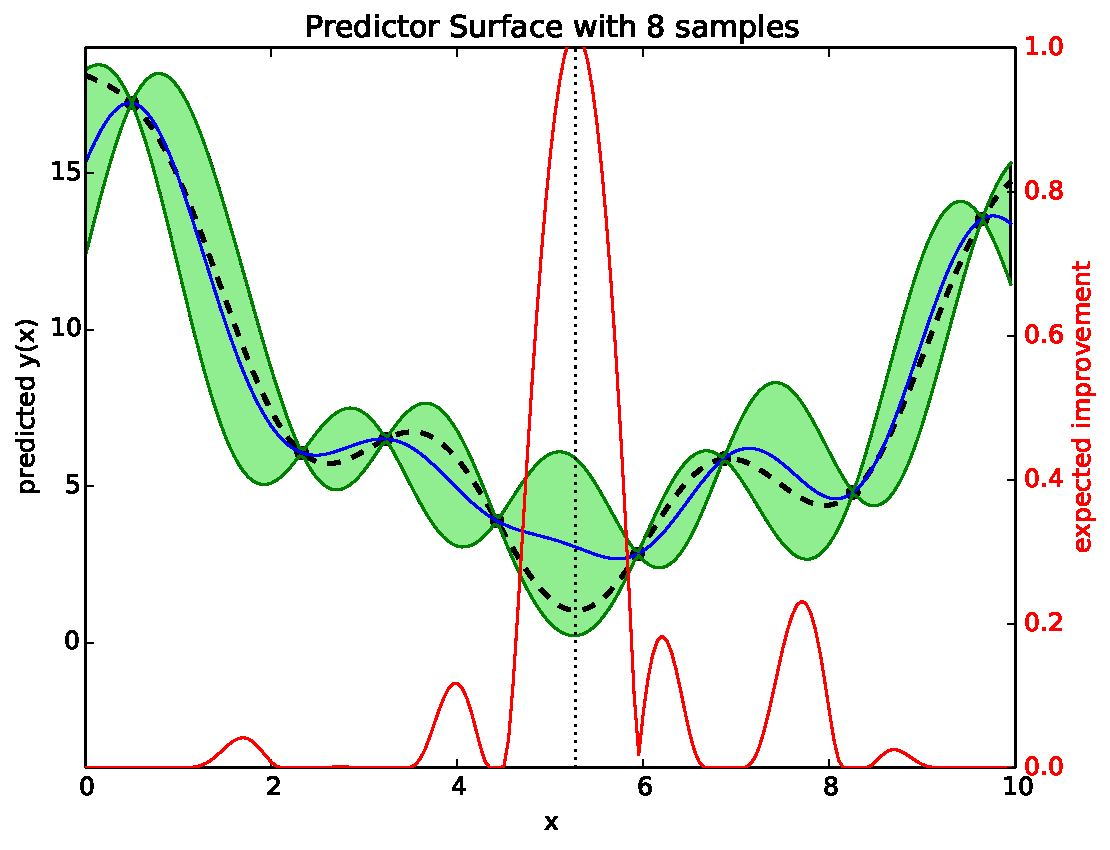
\includegraphics[width=0.5\textwidth]{images/ego_ex/init_w_obj}} \\
\end{tabular}
\caption{The terminating model, produced on the fifth SMBO loop, next to the initial model, with the objective function overlayed.}
\label{fig:explore_exploit}

\begin{minipage}{\textwidth}
\ \\ By the fifth round, plot (a) above, the expected improvement everywhere is so low that the optimization process is complete. The EGO algorithm's halting criteria will be discussed in more depth in the next chapter, but for now it suffices to see that our model predicts very little optimization benefit to taking any further samples.

I have here for the first time overlaid the actual objective function, which has been hidden until now, so the reader can see that this was a successful instance of optimization.\footnote{In my \texttt{smbo} package, \texttt{smbo.tests.smb\_opt} makes it easy to replicate.} For comparison, I have also shown the initial model that was fit five samples ago.

\end{minipage}


\end{figure}









